\section{Phase I Work and Feasibility Study}

The result of the Phase I project is a prototype of the VnV framework. As we will show,
this framework provides all the core functionality required to facilitate in-situ \VV and automated 
documentation generation in numerical simulations. The requirements set by the project team for the Phase I prototype were:

\begin{itemize}
 \item Cross library Support. Most modern numerical simulations rely on a deep hierarchy of numerical simulation tools. For example, BISON, the fuel performance code in the NEAMS toolkit, is built using MOOSE; MOOSE uses libMesh; libMesh uses PETSc; PETSc uses hypre; and hypre uses BLAS. Thus, it is a requirement of the prototype that the system should provide a single interface for in-situ testing in any library linked to the final executable. 
 \item MultiLingual Support: The big three computing languages in high performance computing are C, C++ and FORTRAN. To ensure the system has wide applicability, it is essential that users be able to use the framework in software written in any one of these languages. 
 \item RunTime Configuration: Users should be able run any \VV tests at hard-coded locations in each library without needing to recompile either the executable or the library. The tests themselves should be completely independent from the source code and configurable at runtime. 
 \item Simple Integration: The injection point system should be simple to integrate into existing applications
 \item The framework should automatically generate a highly customizable, publication grade \VV report for each simulation. 
\end{itemize}

These requirements were chosen because they represent the core functionality required to facilitate the development of explainable numerical simulations. That is to say, in demonstrating this functionality, the project team will be able to prove the feasibility of the proposed approach in equipping general purpose numerical simulation toolkits with built in support for end-user solution verification and validation. In what follows we outline the key features of the prototype framework developed in Phase I

\subsection{Injection Points}

At the core of the framework are injection points. Injection points represent locations in a code where \VV testing can take place. Inserting an injection point into an existing function is a simple, three step process; (1) include the ``vv-runtime.h'' header file, (2) place injection points in the code and (3) write the injection point specification.

Figure~\ref{TODO} shows an example code snippet that has been enhanced with VnV injection points. In this case, the original code is taken from the PETSc KSPSolve function and the injection points (shown in red) represent key locations in the code. On the right, we see the injection point specification that describes the state of the code at each injection point.  

\begin{figure}
 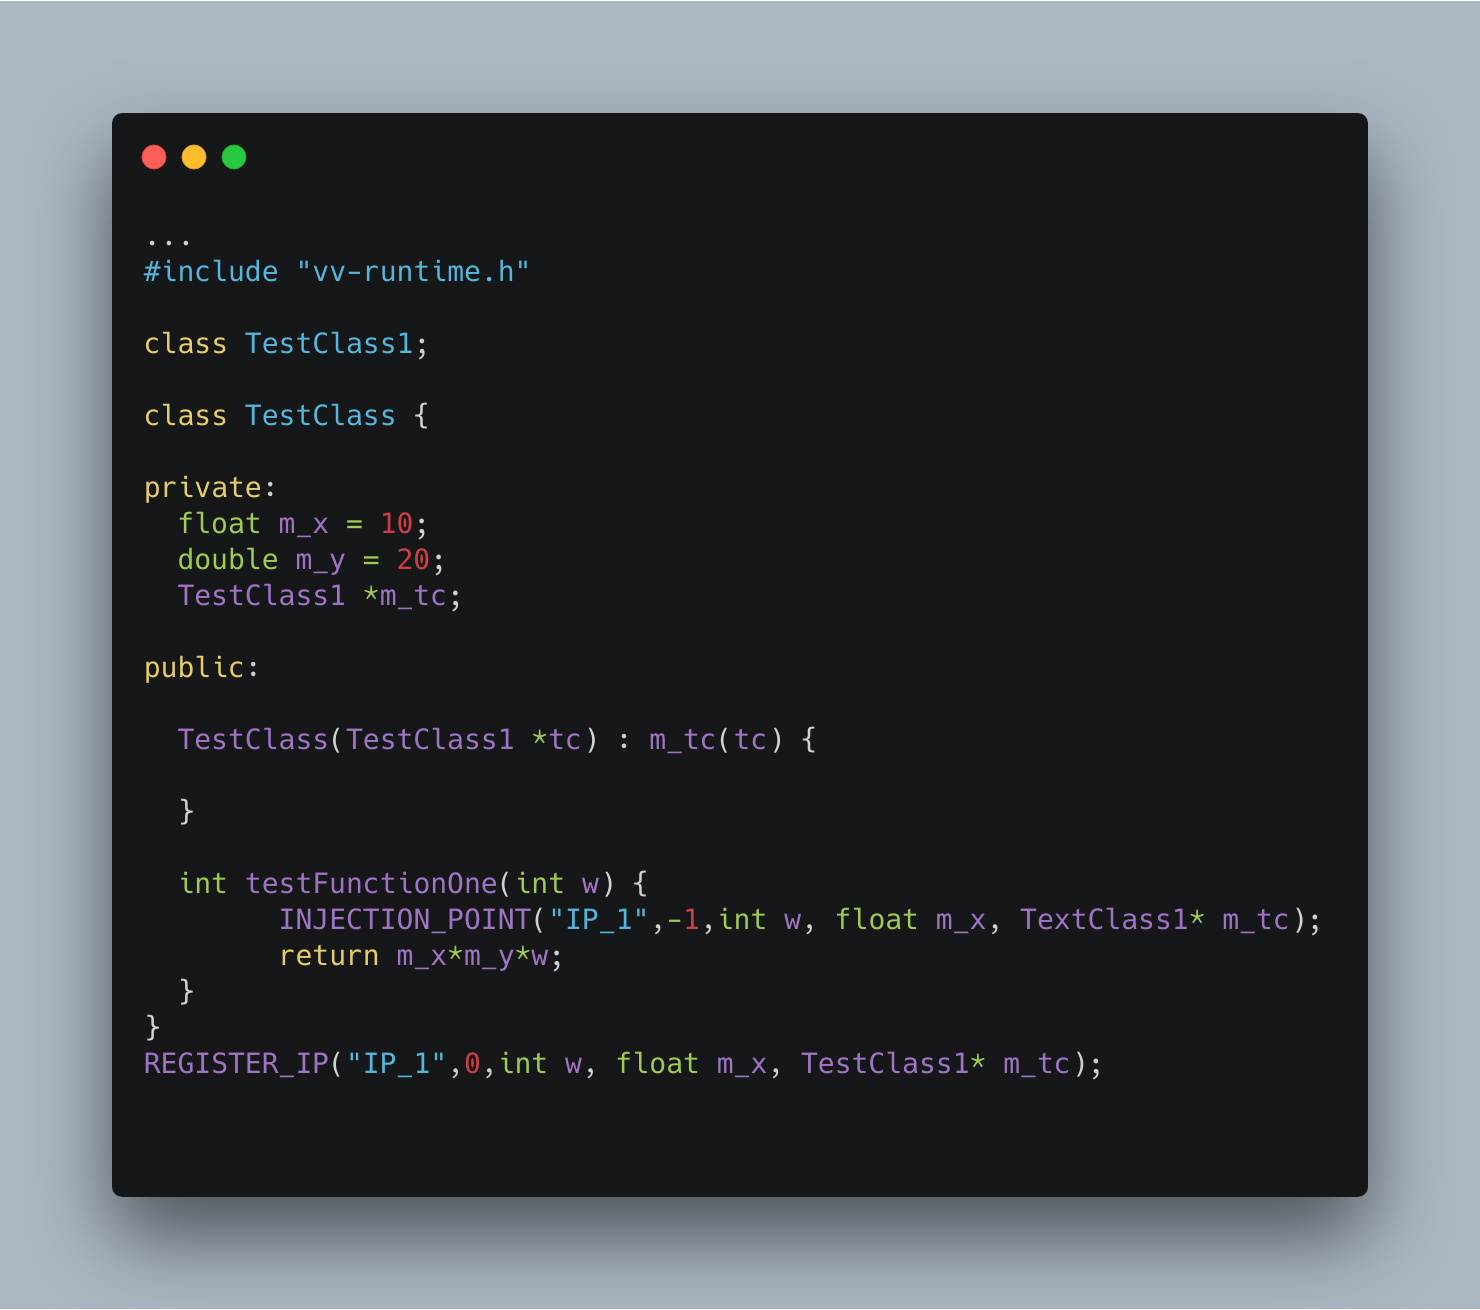
\includegraphics[width=0.45\textwidth]{./Figures/carbon.png}
 \caption{Code Snippet showing a member function enhanced with a single stage injection point. 
\end{figure}


As shown in Figure~\ref{TODO}, declaring an injection point is as simple as calling the INJECTION\_POINT macro. The format for this macro is:

\begin{verbatim} 
INJECTION_POINT( <unique-name>, <stage>, <type> <variable>, <type> <variable>, ... )
\end{verbatim}

The macro is expanded to a variadic C function during preprocessing. Here, the unique name represents the id that will be used to define the injection point in the configuration files and the final reports. This name must 
be unique across all injection points in an executable. 

The stage parameter is an integer value that defines the step that this injection point belongs to. Using this parameter, the developer can set up multi-staged injection point testing. Tests defined on staged injection points stay in scope across 
all stages allowing tests to collect data across multiple code locations. As an example, the injection point on line TODO is a three stage injection point that allows for testing before, after and during a while loop. The phase I prototype supports up to 10000 stages for each injection point, although we have yet to come across a reason for an injection point with more than three or four stages. There are a few restrictions on the stage parameters to ensure efficient data output. First, a single stage injection point should be specified with a stage parameter of -1. A stage parameter less than 1000 should only be used to represent the starting point of a staged injection point. Likewise, a stage parameter greater than 9000 should be used to indicate that this is the last stage in the staged injection point. This allows a staged injection point to have multiple entry and exit points, while also allowing us to automatically handle recursion of injection points.  

The macro supports up to 25 separate variables; although we have not come across cases where more than 5 variables are required. Specifying a variable is as simple 
as writing its type and name. During preprocessing, the macro expands each variable-type declaration as 
\begin{verbatim}
 ..., <type> <name> , ... --> ..., "<type>", (void*) &name , ... 
\end{verbatim}

The runtime module of the framework then maps that void* pointer and the string based type specification to the user specified tests for processing. This is
an obviously risky approach that, when implemented incorrectly, could lead to find memory corruption errors. For example, it would be easy for a developer to
change the type of the variable in the code, but forget to update the string in the injection point declaration. A key goal of the Phase II work will be to 
develop a custom pragma directive that automatically detects the correct type for each variable. 

In C++ codes, the developer can also opt to pre-register the injection point with the runtime module using the REGISTER\_IP macro. The macro uses a feature of object orientated programming languages that allows code in the constructors of static variables to be executed prior to the main function. In this way, one can register certain code elements by simply defining a static variable. Self registration is particularly nice because it allows for run-time detection of the injection points present in the call-graph. That information allows for the automatic generation of a customized test configuration file for each executable. Unfortunately, such a feature is not available in C and FORTRAN, so instead, information about injection points must be determined either by running the full simulation, or by pulling information from the injection point specification files. The custom compiler extension developed in Phase II will address this issue by hardwiring information about the included injection points into the meta-data of the executable or library. 

After an injection point has been declared and optionally registered, the final step is to write the injection point specification. This is specification
is used to populate the content of the final \VV report for each simulation. As shown in Figure~\ref{TODO}, the specification is a YAML file containing a description of the injection point. Writing a YAML specification 
for an injection point is not required; however, the more information entered here, the more informative the final report will be. The fields supported in the YAML specification are:

\begin{itemize}
 \item {\bf description [''``]:} A short description used to describe the injection point in the configuration file
 \item {\bf title:} A descriptive title for the injection point 
 \item {\bf parameters:} A list of the parameters that can be inspected at this injection point
 \item {\bf content:} A markdown formatted string representing the content to be displayed for this injection point in the final report.
 \item {\bf sections:} A map containing the content for any subsections to be displayed under the original content description. Each subsection is displayed
 as a collapseble child or its parents content panel and is included in the overall index of the final report. 
 \item {\bf tests:} A list of tests that could be run at this injection point. 
\end{itemize}

The injection point specification is used during report generation, but is not required when running the executable. This
allows the user to fully customize the final report, even after the \VV testing has been completed. Moreover, the content
component of the specification supports a custom extension of the markdown language that allows for automated generation
of a number of custom data visualization components (described below). 

\subsection{The Testing Interface} 

The second facet of the framework is the \VV testing interface. The development of the 
test interface was based on the idea that tests should be loaded at runtime and defined independently of the source code. To achieve this, the test
interface was built using an C++ plugin pattern. This pattern allows users to develop tests is separate testing modules that can be loaded and configured 
at runtime using an XML configuration file. This allows the users to add or remove tests from injection points located in any linked library without ever 
needing to recompile the executable or any of the libraries. 

The first step in the development of a new VnV test is to create a testing library. The framework includes a library generation script that will automatically build the directory structure and makefiles required to 
build this library. Once the library has been initialized, the user can begin to develop individual tests. 

To simplify the process of writing tests, the VnV framework includes a test generation this script. If the library generation script was used, this script will be available in the src directory of the new testing library. To run this script, the user should provide a unique name for the test and a list of the names and types of parameters that will be supported by the new Test. Using this information, the script generates all the boiler plate code required to implement the IVVTest interface and to handle all the required type-casting. 

From this point, completing the test requires the developer to implement two functions; the delcareIO function and the run\_tests function. 

The declareIO function gives the developer an opportunity to pre-declare the IO variables that will be written by the test. These declarations are not required; however, they allow for optimization in the handling of meta-data in the underlying ADIOS2 IO engine. Readers should look to the ADIOS2 documentation for a detailed description on how to set up and declare IO variables. 

The main function of the test is the runTests function. As shown in Figure~\ref{TODO}, the declaration for this function is

\begin{verbatim}
 TestSuccess run_tests(adios2::Engine &engine, int testStage, <type>* <name>, <type>*, <name>,...)
\end{verbatim}

Here, testStage is an integer representing the stage that the test is currently in. A test can support as many stages as there are integers. For example, 
the test shown in Figure~\ref{TODO} supports three stages; one for setup, one for data collection and one for finalization. As will be shown below, the test 
stages are mapped to injection point stages at runtime using the test configuration file. 

Data output can occur at any point in the run\_tests functions. The core runtime module ensures that each test stage is completed in a unique ADIOS2 step. This allows for efficient 
compartmentalization of the test output and makes post-processing significantly easier. As in the delcareIO function; data output is completed directly in ADIOS through the 
ADIOS2 read/write API. As an example, the test in Figure~\ref{TODO} writes a data array to the output during the finalization stage of the test. 

The final step in writing a test is to write the test specification. As with injection points, this specification acts as a template for the 
content to be shown in the final report. The specification is written in a YAML file and supports writing content using the VnV extended markdown format. As will be described 
in the following section, this extended markdown specification allows for direct querying of the data output during each stage of a \VV test. In this way, the user can 
create a generic, data agnositc template for the \VV test output that will be populated with data during post-processing. 

\subsubsection{Variable Modifiers}

In addition to tests, the VnV framework also provides support for pluggable variable modifiers that can be used to 
map injection point parameters into formats that can be consumed by the tests. These Test modifiers are developed using 
the same plugin based C++ pattern used to define the tests and can be included in seperate Modifier libraries or as seperate 
components in existing testing libraries. Some examples of modifiers implemented during the Phase I testing include; a dereference modifier
that dereferences a pointer variable; an array access modifier that pulls out the $n$'th element from an array variable; and a PETScPC modifier that
uses the KSPGetPC function to provide direct access to the internal preconditioner. 


\subsection{Extended Markdown Format for Numerical Simulations} 

The Extended markdown format for numerical simulations, MD-XNS,  was developed for the VnV project as a highly customizable system for automatically processing 
the results obtained from numerical simulations into interactive, informative HTML/JS web pages. The extension itself was built using py-markdown, an open source 
python library for converting markdown files into html.

In addtion to standard markdown commands, the MD-XNS format supports custom post-processing commands of the form [VV::<name>={...}], where name is the name of 
the component the user would like to insert and {...} represents a dictionary of configuration options. 

The Phase I prototype supports a range of custom processing functions including 
\begin{itemize}
\item Table: The table command inserts an interactive, sortable, searchable table into the final html document. The user can populate the table by entering the information
manaully, by providing the name of a csv file, and/or by providing a list of numpy arrays. 
\item Chart2D: The Chart2D command inserts an interactive Charts.JS chart into the document. The entire array of Charts.JS charts are available through this component, including bar, 
line, scatter and pie charts. In each case, the chart is configured using a python dictionary entered directly into the markdown. 
\item VTPView: The VTPView command uses VTK.js to insert interactive 3D visulization of a .VTP files in the final document. 
\item PostPro: The PostPro function allows the user to set up post-processing scripts for execution during the report generation phase. In this way,
users can write simple scripts that parse the data into formats more suitable for use in any of the other data visualization components. 
\item ThreeJs: The ThreeJS command provides another approach for integrating three dimensional visualization in the final report, in this case using three.js for rendering. This 
component is particularly usefull for viewing meshes. 
\end{itemize}
Figures~\ref{TODO} show examples of the html web-components supported using the MD-XNS format. The key functionality of the MD-XNS format lies in its ability to directly interact with data stored in ADIOS2 bp3 steps. For example, Figure~\ref{TODO} shows a MD-XNS file that automatically populates a plot using an array available at an ADIOS2 step under the variable name ``data''. In this way, MD-XNS allows users to write generic templates that can be populated with data during processing. This is particularly nice for \VV injection points and \VV tests because each test knows extactly what data can appear during each call to the overall testing algorithm. 


\subsection{The VnV Runtime Module}

The VnV runtime module is the driving force behind the framework. This module contains all the functionality required  to detect the injection points, parse the
configuration file, setup the ADIOS IO engine, load the external testing libraries and run all the tests. Despite this, configuring a simulation to use the VnV 
framework is a simple, four step task; (1) include the header file, (2) Call the VVInit(<input-file>) function at the start of main, (3) Call the VVFinalize function
before exiting, and (4) link the VnV library to the main library along with any required sublibraries. 

Once the configuration has been completed, users will be able to control the entire VnV process through the input file. The Phase I prototype 
uses a XML based input file. Figure~\ref{TODO} shows the XSD specification for the input file. The VnV toolkit uses a  modified version of Xsd2Cpp to generate 
a C/C++ DOM parser for the XML file. 

The key sections of the input file specification are:
\begin{itemize}
 \item The Simulation Information. The simulation information section is where the user can provide information at the simulation. 
 \item The Testing Libraries. The testing libraries element is used to define external testing libraries that will be used in the final executable. 
 \item The Introduction. The introduction element a
\end{itemize}



\subsubsection{Automated Report Generation}

In addition to the injection point system, the project team also developed an initial prototype for automatically generating
the final report. After accessing the strengths and weaknesses of multiple different approaches, the project team
decided on a server-less HTML/JS format generated using a custom extension of the markdown format. The primary benefit of this approach is portability - the report can be displayed in any web browser - but other benefits include interactive components, non-linear data presentation and high levels of customization. Moreover, the server-less nature of the HTML web-page allows for direct publication on any static web hosting service (github.io, AWS S3, etc.). 

Figures~\ref{TODO} show screen-shots of a sample VnV report generated using a set of toy testing libraries. The main layout consists of three components; the carousel, the index and the content. The carousel is an optional component that can be used to highlight important results of the simulation. It accepts up to ten pictures, each with its own custom caption. Simpler static headers are also possible. The index and content are generated automatically based on the VnV output file. Each node in the index represents an injection point encountered during the simulation. As such, this index represents a coarse grained view of the simulations call stack. At the top of each injection point section is the injection point content as specified in the injection point specification. Following this is the output of each test completed at the injection point. Last is the list of children. These children represent injection points that were initialized between the first and last step of a staged injection point. A live version of this sample VnV report will be available at http://www.rnet-tech.net/VV/sample.html until the date of award notification. 




\subsubsection{ Demonstration in a Moose Application } 
To demonstrate the utility of the method, the project team placed several injection points 
in the main function of a MOOSE example ``ex01'', one injection point in the PETSc Initialize function and 
one injection point in the PETSc Finalize functions. This is an extremely simple example that 
did not test the full limits of the new API; however, it did act to verify that the phase I prototype 
can be used to can be used to perform in-situ verification and validation in a across multiple libraries 
through a single interface. A screenshot of the final \VV report obtained from those tests is shown in the 
final report. 

In summary, during Phase I, the project team created a functioning prototype of the VnV framework that provides:
\begin{itemize}
 \item A clean mechanism for inserting injection points in existing codes
 \item A simple interface for defining custom tests 
 \item A customizable approach for automatic post-processing of testing data and injection points
 \item A python based report generation code that automatically creates an interactive server-less web report based on the VnV output.
\end{itemize}

As will be described in the workplan, the goal of the Phase II project will be to take this initial prototype and extend, harden and 
optimize it such that it can be efficiently used in high performance computing applications. 







\section{Phase I Task Completion}
With regard to the proposed Phase I tasks, our achieved objectives are as 
follows:

\subsection{Task 1: Automatic Execution on Cloud}
The effort needed to implement a standalone Core with Remote OSGi services, 
turned out to be larger than anticipated since extricating relevant 
dependencies took most of the time. Since ICE is already capable of launching 
remote jobs and we have the standalone Core instance, we believe we are very 
close to realizing this with the Nek5000 form in Vaadin.

We will focus on connecting the CloudBench UI to the standalone Core instance 
and validating the connection.

\subsection{Task 2: Design and Development of Local Databases}
Our initial focus will be on Nek5000 as it is an open source project and does 
not face the same ITAR restrictions that other tools would impose. When we 
validate our prototype and specialize CloudBench towards CloudBench:NE, we will 
increase our portfolio of supported codes. The development of such a database 
would be more appropriate at that time, which we would revisit.

Also it is likely that the codes could be run on a myriad of hardware 
configurations. Trying to compile and store binaries for each combination of 
hardware configurations would be too unwieldy. We would store only a few 
standard binaries but focus more on automatically compiling the installed 
source codes, so that it better suites that particular environment.

\subsection{Task 3: Web Portal Prototype and Promotion}
Our efforts outlined in Section~\ref{sec:cloudbench_ui_dev} describe our web 
portal prototype based on Vaadin. We believe that our CloudBench prototype will 
provide an intuitive interface and feel across all platforms which will 
encourage the adoption in various scientific communities. The targeted industry 
is the businesses and other institutions (e.g., government research labs, 
universities, energy companies) that perform large-scale numerical modeling and 
simulation. The end users are the engineers and researchers who carry out 
numerical simulations (e.g., to use simulation to better understand their 
designs before prototyping).

% taken from Commercialization
The business model for CloudBench will be to sell Cloud accounts and 
preconfigured simulator access (on Cloud resources) directly to users, to sell 
software licenses for private servers for installation on third-party systems, 
and contractual services to develop support for additional clusters (private or 
public), simulation tools, and features. The potential NEAMS users (GE Hitachi, 
EPRI, Areva, DOE Labs, NASA divisions etc.) will be our initial customers and 
end users.

